
%%%%%%%%%% Conference Latex Template for the university center of Tipaza - Algeria
%%%%%%%%%% created by F.CHABNI




\documentclass{paper}
\usepackage{ctex}
\usepackage{geometry}
\usepackage{graphicx}
\usepackage{amsmath}
\usepackage{cite}
\usepackage{subcaption}
\usepackage{booktabs}
\title{自主移动车实现研究综述}
\author{邱璟祎, 周俊豪, 张峻瑜\\
  (按姓名首字母排序)
}
\geometry{a4paper,scale=0.8}
\begin{document}
\maketitle
\tableofcontents
\newpage
\section{引言}

\part{自主移动车文献综述}
\label{sec:label}


\section{机械设计研究综述}
\subsection{运动方式}
\label{subsec:label}
目前自主移动车的运动方式主要分为轮式和履带式,下面将分别论述这两种方式的特点。
\subsubsection{轮式运动}
\label{subsec:label}
轮式运动是最常见的自主移动车的运动方式,其特点是使用一组或多组轮子进行移动,可以采用常规的轮胎或全向轮设计,适用于平坦、结构简单的环境,灵活程度比较高,结构简单、可控性强、安全性好。按照驱动方式进行分类又可以分为单驱轮式、双驱轮式和多驱轮式。单驱轮式通常适用于三轮式AGV,双驱轮式则通常适用于四轮式AGV,这两类驱动方式的特点是整个AGV只有一部分车轮具有驱动力,可以减少驱动电机的数量,减少车体重量,节约内部空间;但采用这类驱动方式的小车往往由于配重不均匀会出现非驱动轮一侧抓地力不足的问题,小车转向容易出现问题。多驱轮式的AGV的所有车轮都和驱动电机相连,驱动能力更强,配重更加均匀,但是灵活性有所降低。
\subsubsection{履带式运动}
\label{subsec:label}
履带式运动的AGV对地面的单位压力小,摩擦力较大,抓地力较好,适合在雪地、山坡等比较恶劣的地面环境下工作,能承受比较大的负载,但是成本比轮式AGV高很多,速度比较慢。
\subsection{转向方式}
\label{subsec:label}
目前已有的AGV中,转向方式大部分都可以归结为差速转向和麦克纳姆轮转向两大类,下面将分别进行叙述
\subsubsection{差速转向\cite{chasu}}
\label{subsec:label}
假定前轮和后轮都是驱动轮,则参考阿克曼(Ackerman)转向几何学原理,即在汽车转向时4个轮胎都近似围绕一个中心点旋转以保证汽车的行驶稳定性。把汽车的形心作为质心,并且忽略路面情况变化等的影响,可得出四轮驱动差速转向小车的运动学模型如下图所示。
\begin{figure}[ht]
  \centering
  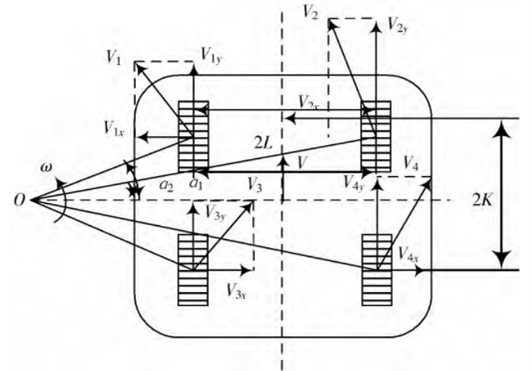
\includegraphics[width=0.5\textwidth]{figures/chasu.png}
  \caption{差速转向受力分析}
\end{figure}
$\alpha_1$和$\alpha_2$分别为前左轮和后左轮,前右轮和右轮的转角;2L 为左右轮距离; 2K 为前后轮轴距;$v$和$\omega$分别为车子质心的线速度和角速度,$V_1,V_2,V_3,V_4$分别为各个轮中心的实际运动方向。由图 可以得出各速度和转角的关系:
\[\begin{gathered}
V_{1}=\omega R_{1}=\omega\frac{K}{sin\alpha_{1}}\leftarrow \\
V_{2}=\omega R_{2}=\omega\frac{K}{sin\alpha_{2}}\leftarrow \\
V_{3}=V_{1}=\omega\frac{K}{sin\alpha_{1}}\leftarrow \\
V_{4}=V_{2}=\omega\frac{K}{sin\alpha_{2}}\leftarrow \\
V_{1y}=V_{1}cos\alpha_{1}= \omega\frac{K}{tan\alpha_{1}}=\omega(R-L)^{\leftrightarrow}\\
V_{2y}=V_{2}cos\alpha_{2}= \omega\frac{K}{tan\alpha_{2}}=\omega(R+L)^{\leftrightarrow}\\
V_{3y}=V_{3}cos\alpha_{1}= \omega\frac{K}{tan\alpha_{1}}=\omega(R-L)^{\leftrightarrow}\\
V_{4y}=V_{4}cos\alpha_{2}= \omega\frac{K}{tan\alpha_{2}}=\omega(R+L)^{\leftrightarrow}
\end{gathered}\]
式中$R=\frac v\omega $。

则电机的角速度为:$\omega_n=\frac{V_{ny}i}r,n=1,2,3,4$

式中$i$为减速器的减速比,$r$为车轮半径。


\subsubsection{麦克纳姆轮转向\cite{mac}}
\label{subsec:label}
麦克纳姆轮移动平台具有平面上3个自由度的移动能力,依靠4个轮子各自不同转速的相互配合来实现全向移动,每一个轮子的运动都对整体的运动方向和速度大小有着很大的贡献。麦克纳姆轮它与普通轮之间的主要区别就在于它的圆周上分布有若干数量的辊子,这些辊子的轴线与轮子的轴线呈一定的夹角(如45°),辊子的外廓线所形成的包络面和轮的原始圆周面重合,这样保证了辊子能与地面一直保持接触这些辊子还可以自由转动,这使得轮子只受到地面对辊子轴向上的力,而地面对辊子的圆周力则变为了滚动摩擦,可以近似看为零。因此,轮子与地面的接触力不再是沿轮子的圆周方向,而是与它呈一定的夹角,所以这种轮子可以在一个方向上受到摩擦力的驱动,而在另一个方向上自由移动。由4个这样的轮子便可以组合出不同的受力情况,从而使移动平台可以实现平面上3个自由度的移动。
\begin{figure}[ht]
  \centering
  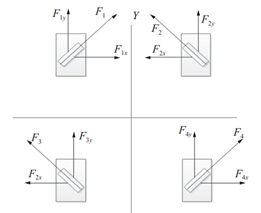
\includegraphics[width=0.5\textwidth]{figures/mac.png}
  \caption{麦克纳姆轮受力分析 }
\end{figure}

用$R$表示全向轮轴心到轮外廓圆周面的距离即轮的半径;$V_i$表示第$i$轮的速度;$\alpha$表示辊子轴线与全向轮轴线夹角;$\omega_i$表示全向轮绕轮轴的转速;i=1,2,3,4,分别代表左前轮、右前轮、左后轮、右后轮。联立可得矩阵方程:
\[ V_i=\begin{pmatrix}R\\4\end{pmatrix}\begin{bmatrix}1&1&1&1\\\tan\alpha&-\tan\alpha&-\tan\alpha&\tan\alpha\\-\frac{1}{l_0}&\frac{1}{l_0}&-\frac{1}{l_0}&\frac{1}{l_0}\end{bmatrix}\begin{bmatrix}\omega_1\\\omega_2\\\omega_3\\\omega_4\end{bmatrix}\leftarrow  \]
式中$l_0=$W+ Lcos$\alpha$,其中 W 为移动平台宽度,L 为其前后轮轴距;而$\alpha$取
$45^{\circ}$,其正负号已被提出,不再区分正负。逆运动学方程为:
\[\begin{bmatrix}\omega_1\\\omega_2\\\omega_3\\\omega_4\end{bmatrix}=\text{K}\begin{bmatrix}V_y\\V_x\\\omega\end{bmatrix}=\begin{pmatrix}\frac{1}{R}\end{pmatrix}\begin{bmatrix}1&cot\alpha&-l_0\\1&-cot\alpha&l_0\\1&-cot\alpha&-l_0\\1&cot\alpha&l_0\end{bmatrix}\begin{bmatrix}V_y\\V_x\\\omega\end{bmatrix}\leftarrow \]
总的来说,麦克纳姆轮转向具有高效率、高灵活性的特点。
\subsection{抓取机构}
\label{subsec:label}
机械臂末端的抓取机构可以采用机械手爪、吸盘和仿生结构三种形式,它们具体的特点如下:
\subsubsection{机械手爪}
\label{subsec:label}
机械手爪按照驱动方式不同可以分为气动驱动、电动驱动、液压驱动、电磁驱动和热驱动五种方式。气动驱动使用压缩空气来控制手爪的开合,成本较低,响应速度快,但是需要压缩空气源,且控制精度相对较低。电动驱动使用电机作为动力源,通过齿轮、皮带或丝杠等机械结构传递动力,控制精度高,力矩输出稳定,但是结构可能较为复杂,成本相对较高。液压驱动利用液压系统产生的动力来驱动手爪,可以产生较大的力,适合重载应用,但是需要液压泵和管路系统,维护成本较高。电磁驱动通过电磁铁产生的磁力来控制手爪的动作,响应速度快,结构简单,但是力量输出可能受限于磁场强度。热驱动利用热胀冷缩的原理来驱动手爪,可以实现柔性抓取,但是响应速度慢,适用范围有限。

\subsubsection{吸盘}
\label{subsec:label}
吸盘可以分为磁力吸盘和真空吸盘两大类。磁力吸盘的体积小,自重轻,吸持力强,广泛应用于钢铁、机械加工、模具、仓库等搬运吊装过程中对块状、圆柱形导磁性钢铁材料工件的连接,可大大提高工件装卸、搬运的效率,但是对所抓取的物品有磁性的要求。真空吸盘原理简单,操作相对容易,但前提是要保证所抓取物品表面足够平整光滑,此外还需要注意对于吸盘盘面的清洁与保护,防止污渍与腐蚀,对于后期维护保养的要求较高。
\subsubsection{仿生结构}
\label{subsec:label}
面对外形较为复杂的物品,可以采用多指灵巧手的仿生结构作为夹持机构。在众多仿生结构中,人形手模仿人类手的外形和运动自由度,通常具有多个关节和独立运动的手指,可以实现复杂的抓取动作,如捏取、旋转和握持,适用于需要高度灵活性和精准控制的应用场景。柔性夹持器采用柔软材料制成,例如硅胶或弹性聚合物,可以根据物体的形状和尺寸进行自适应的夹持,能够温和地处理各种形状的物体,腱驱动手使用类似于人类手臂的腱结构来驱动手指的运动,通过线缆或弹性材料控制手指的张合,提供较好的力量和运动控制,可以实现较强的夹持力和灵活的手指运动。不完全驱动手的手指之间可能共享某些驱动元件,这种设计可以减少驱动部件的数量,提高了系统的可靠性和节省成本。生物启发自适应夹持器借鉴动物或昆虫的夹持机制,如螯虎或章鱼的吸盘结构,实现了在不同形状和尺寸的物体上的高效夹持能力和自适应性。


\section{循迹研究综述}
\subsection{传统而有效的方法\cite{intro2023robot}}
\label{subsec:label}
\subsubsection{传感器:红外传感器、光敏电阻等}
\label{subsec:label}
红外传感器、光敏电阻等传感器实际上提供的传感能力是同质化的,此处以红外传感器为例介绍传统方法所用的传感器。

红外传感器是各种机器人比赛中最常见的传感设备。红外传感器可以发射红外光并接收反射光,根据反射光的强度输出电压。输出电压在经过有着固定基准值的电压比较器处理后将输出逻辑电平,便于控制器处理。
\begin{figure}[ht]
  \centering
  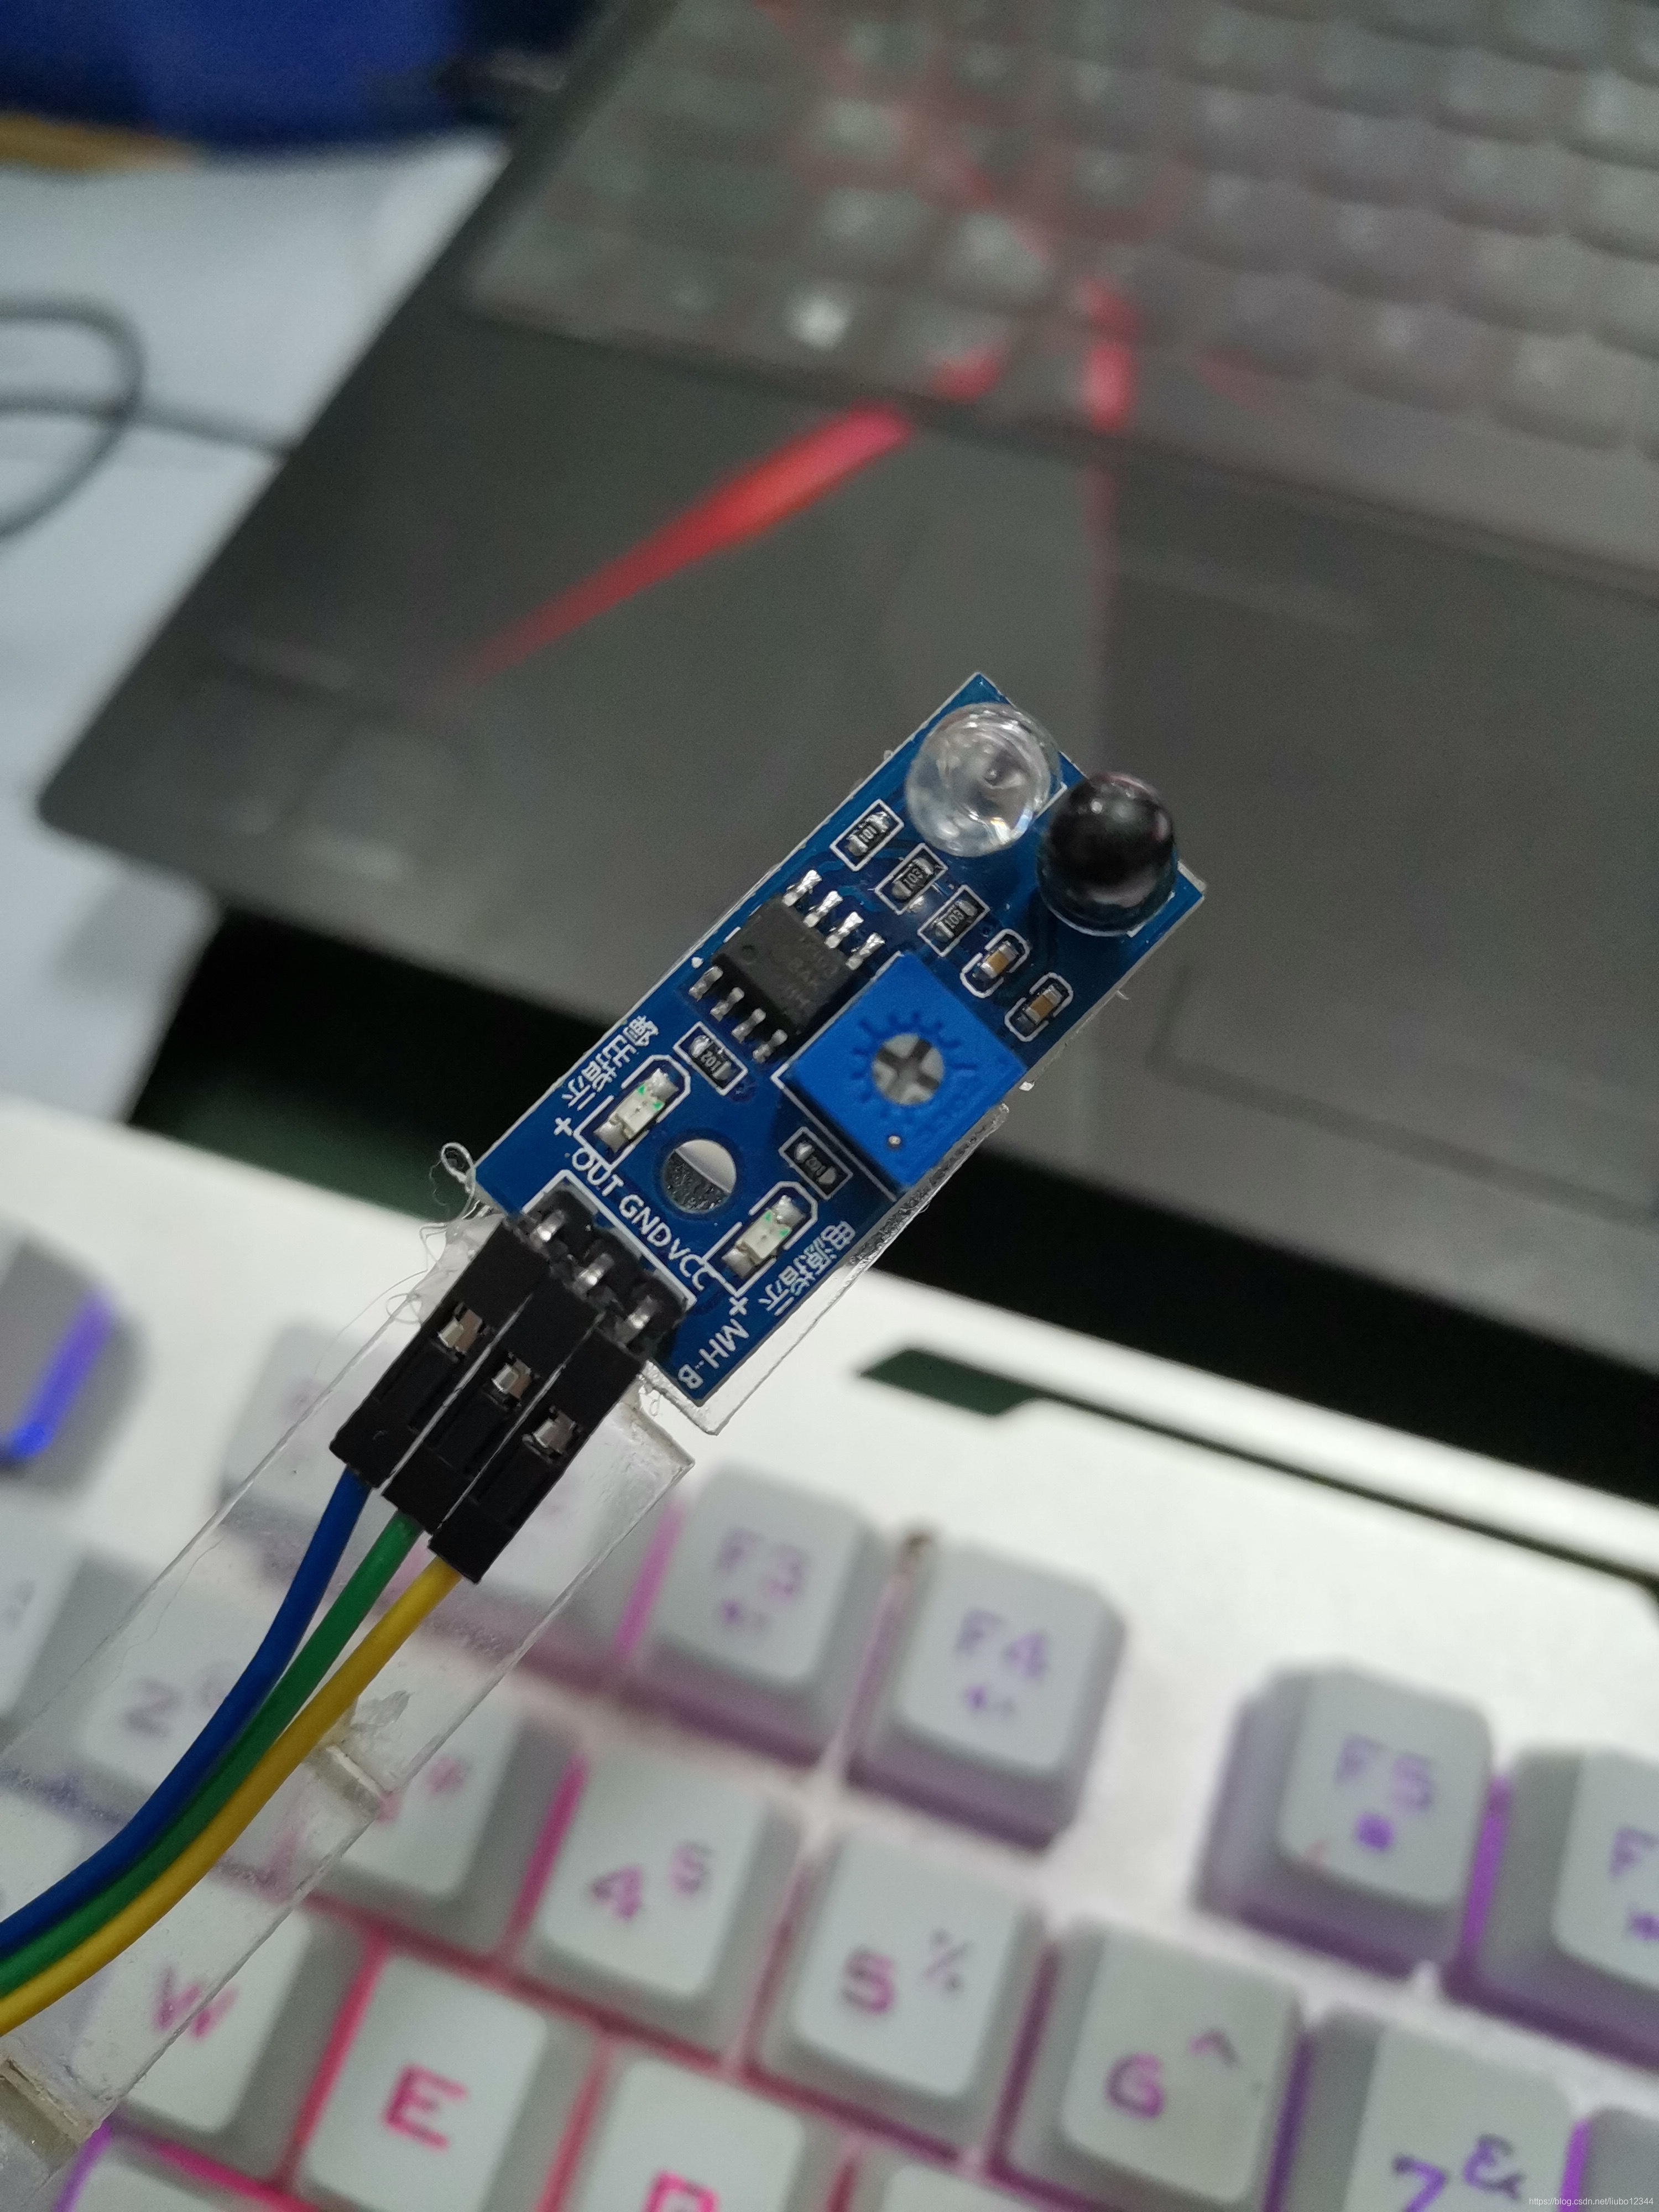
\includegraphics[width=0.5\textwidth]{figures/sensor.jpg}
  \caption{ 常见的红外传感器}
\end{figure}

常见的使用方案是在循迹车的前方布置对称的红外传感器。当线出现在红外传感器的正下方,它便会给控制电路采取行动的信号。例如当需要小车保持在黑色边线的赛道内时,如果侧边传感器有信号,则控制向另一个方向转弯。这种实现非常简单直观。

然而红外传感器的缺陷在于其只能给出是否检测到线的信息,而不能给出线的远近、角度信息,这使得它无法实现更加复杂和高效的控制算法。
\subsubsection{算法:从if-else到PID}
\label{subsec:label}
空间上离散的点观测传感器实际上提供了有限的状态数,只要根据状态给定行为就可以完成简单的控制。这只需要简单的if-else逻辑就能实现。但这样简单的方法代价是不够灵活,并且一个固定的控制指令并不能总是实现最优的控制。实际上的小车可能会困在反复地左右摇摆中浪费大量的时间和能量。

如果我们有一个点观测传感器组成的阵列例如线性CCD(含有128个光敏电阻)或者进一步线性传感器,我们可以离散地或连续地得到与线之间的距离。如使用线性CCD元件\cite{CCD},将黑线在CCD正中间认为是基准值,数值从右向左增加,误差定义为当前值与标准值的差。这使得我们能够向循迹算法中引入PID。设定一个中间状态作为PID的基准,传感器阵列得到的距离可以作为PID的误差。利用PID控制两轮的转速差,使其小车保持在中间状态,可以实现更平滑、更快的循迹。

\subsection{更灵活高效的新方法}
\label{subsec:label}
\subsubsection{计算机视觉\cite{opencv}}
\label{subsec:label}
采用计算机视觉方法可以为系统获得更广的感受野和更复杂的信息。传统的方式是首先获取图像,把图像转化成灰度图再进行二值化,得到黑白图像。黑色点的平均横坐标反映了循迹线的倾斜程度。据此,可以设置阈值或PID使得小车保持巡线。
\begin{figure}[ht]
  \centering
  \caption{经过灰阶化-二值化的图像}
   \begin{subfigure}[b]{0.3\textwidth}
     \centering
     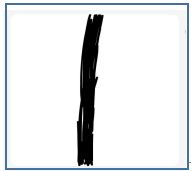
\includegraphics[width=\textwidth]{figures/straight.png}
     \caption{直行}
     \label{fig:label}
   \end{subfigure}
   \hfill
 \begin{subfigure}[b]{0.3\textwidth}
   \centering
   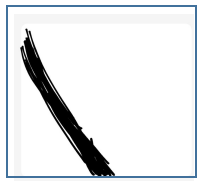
\includegraphics[width=\textwidth]{figures/left.png}
   \caption{左转}
   \label{fig:label}
 \end{subfigure}
 \hfill
 \begin{subfigure}[b]{0.3\textwidth}
   \centering
   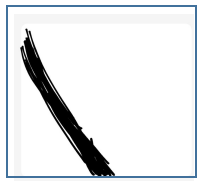
\includegraphics[width=\textwidth]{figures/left.png}
   \caption{右转}
   \label{fig:label}
 \end{subfigure}
 \hfill
\end{figure}

但对于单片机而言,矩阵的高运算量带来的时间消耗限制小车的移动速度。这时我们就需要对算法进行优化。首先并不是视野中的所有信息都需要被纳入决策中,我们实际上只需要考虑距离小车较近的部分,可以裁剪掉多余的部分。接着,每一帧图像中黑线的趋势可以间隔采样来获取,而不是全部计算。

\begin{figure}[ht]
  \centering
  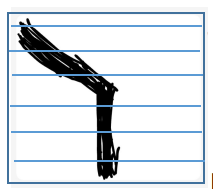
\includegraphics[width=0.5\textwidth]{figures/jumpscan.png}
  \caption{间隔采样 }
\end{figure}

卷积也可以有效地减小需要遍历的矩阵。采用矩阵池化来用局部特征替代整体特征。池化实际上是将矩阵分成多个与卷积核一样大的小块,使用小块内元素的特征(最大值或者平均值)来代替这个区域。
\begin{figure}[ht]
  \centering
  \includegraphics[width=0.5\textwidth]{figures/pooling.png}
  \caption{最大值池化}
\end{figure}


\subsubsection{强化学习}
\label{subsec:label}
2024年Yu Cao等人进行了深度强化学习循迹机器人的理论研究\cite{cao2024path}。他们将机器人与线路的横向偏差、机器人与路径之间的方向误差、机器人的速度和角速度等信息作为状态,而将机器人速度的变化率作为行动。在奖励函数中纳入与误差成正比的惩罚、与速度成正比的奖励以及惩罚机器人在困难弯道停下的参数。

\begin{figure}[ht]
  \centering
  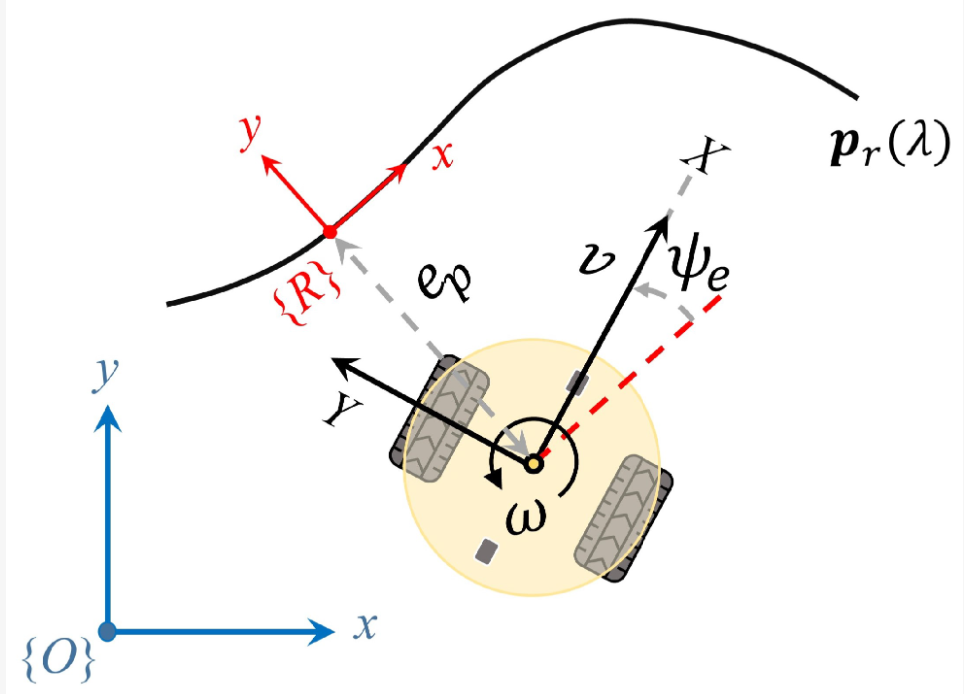
\includegraphics[width=0.5\textwidth]{figures/state.png}
  \caption{状态定义物理量\cite{cao2024path}}
\end{figure}

\[ r\left(t\right)=-k_{1}\left|e_{p}\left(t\right)\right|+k_{2}v\left(t\right)\left(1-\frac{1}{e_{tol}}\left|e_{p}\left(t\right)\right|\right)-k_{3}F\left(t\right) \]
在随机生成的环境中进行了50万次交互之后,机器人的路径实现收敛。相比传统的PP控制方法,采用深度强化学习的机器人有了自适应的速度控制能力,可以适应不同曲率的路径,还有相当不错的泛化能力,在随机生成的不同路径中均有优秀的效果。

根据现实硬件情况在Webbot中建模并进行虚拟环境的预训练,再将完成训练的模型下载到实际小车中,就可以实现该方法的实际运用。
\section{避障研究综述}
\label{sec:label}



\section{讨论}
\section{结语}


\bibliographystyle{IEEEtran}
\bibliography{references}

\end{document}

%%% Local Variables:
%%% mode: LaTeX
%%% TeX-master: t
%%% End:
